\documentclass[11pt]{article}
\usepackage{fontspec}
\setmainfont{STIX Two Text}[BoldFont={STIX Two Text Bold},ItalicFont={STIX Two Text Italic Italic},BoldItalicFont={STIX Two Text Italic Bold Italic}]
\usepackage[margin=1.05in]{geometry}
\usepackage{graphicx,booktabs,caption,microtype,enumitem}
\usepackage[hidelinks]{hyperref}
\captionsetup{font=small,labelfont=bf}
\setlist{itemsep=2pt,topsep=4pt}
\linespread{1.08}

\title{\textbf{A Dawn Calendar in Eight Parts}\\[4pt]
\large Measuring the Nineveh Planisphere (K\,8538) with Cribs}
\author{Logan C. Ross}
\date{29 October 2026}

\begin{document}
\maketitle

\begin{abstract}
\noindent
The round clay tablet K\,8538 from Ashurbanipal's library at Nineveh has been read as a sky at sunset,
a magic object, a single night's horizon, and the record of an asteroid strike. No reading has been
measured against chance. This paper does so. Known identifications on the tablet serve as cribs,
in the cryptanalytic sense, and every published reading is scored under the same rules against
thousands of random tablets, with each rule written down and hashed before the run that used it.
One format outperforms all the others: a calendar of eight periods, each marked by the
constellations first seen rising before dawn at Nineveh. On the four cribs shared by every reading
it scores 2.0\%, against 8.7\% for the best published alternative. A fifth crib, fixed by a
prediction locked in advance and then passed, brings the result to \textbf{0.64\%} of
10{,}000 random tablets, stable from 1500 to 400\,BCE. With the modern identification of one
constellation, all five cribs fall exactly in their slices (0.48\%). The tablet is read here as an
administrative calendar of eight 45-day periods within the 360-day administrative year. Why the
administration counted in eighths is not yet known.
\end{abstract}

\section{A century of readings}

K\,8538 is a disc about 14\,cm across, divided by four diameters into eight equal slices and covered
with star marks, drawn figures, constellation names, rows of repeated signs, and one row of numbers
\cite{king1912,cdli}. It is the only eight-segment circular diagram known in cuneiform; every other
has twelve \cite{monroe2022}.

\begin{itemize}
\item \textbf{Bosanquet and Sayce (1880)} gave the first transcription and read the disc as a drawing
of the sky, with its repeated signs as a 48-part scale \cite{bs1880}.
\item \textbf{King (1912)} published the hand copy on which all later work rests \cite{king1912}.
\item \textbf{Weidner (1915)} read the tablet sector by sector from a photograph. He found the named
constellations ``in the correct order'' but not in exact positions, placed the large figure of
the first slice at the winter solstice, and concluded that the object served magic or divination
\cite{weidner1915}.
\item \textbf{Koch (1989)}, as reported secondhand, read a static horizon map for the night of
3--4 January 650\,BCE \cite{koch1989}.
\item \textbf{Bond and Hempsell (2008)} read a dawn observation of an object on 29 June 3123\,BCE and
linked it to the Köfels landslide in the Alps \cite{bh2008,bristol2008}. Seifert and Lemke proposed a
rival impact date, 22 September 2193\,BCE \cite{sl2019}.
\end{itemize}

\noindent Each reading saw something real. None was scored against what chance alone would produce.

\section{Back to the sources}

The working sources are King's plate at full scan resolution, the 1880 transcription, and Weidner's
reading, which corrects several of the 1880 glosses: Orion stands in the fourth slice, not the fifth;
the line of seven holes belongs to APIN; the sign \emph{hu} means ``bird'', not ``cubit''. The plate
itself is drawn true: its dividers lie within 0.6° of 0°, 45° and 90°.

Two instrument checks came before any hypothesis. Fake tablets built from known skies showed that
star labels in eight 45° sectors cannot date a tablet: the best-scoring band spans about 3{,}000 of
the 3{,}500 years searched, so no single-night reading can rest on the star layout alone. Sky
positions come from the Swiss Ephemeris with the JPL DE441 files \cite{swisseph,de441}, checked against
an independent model to within arcseconds for most bodies.

\begin{figure}[t]
\centering
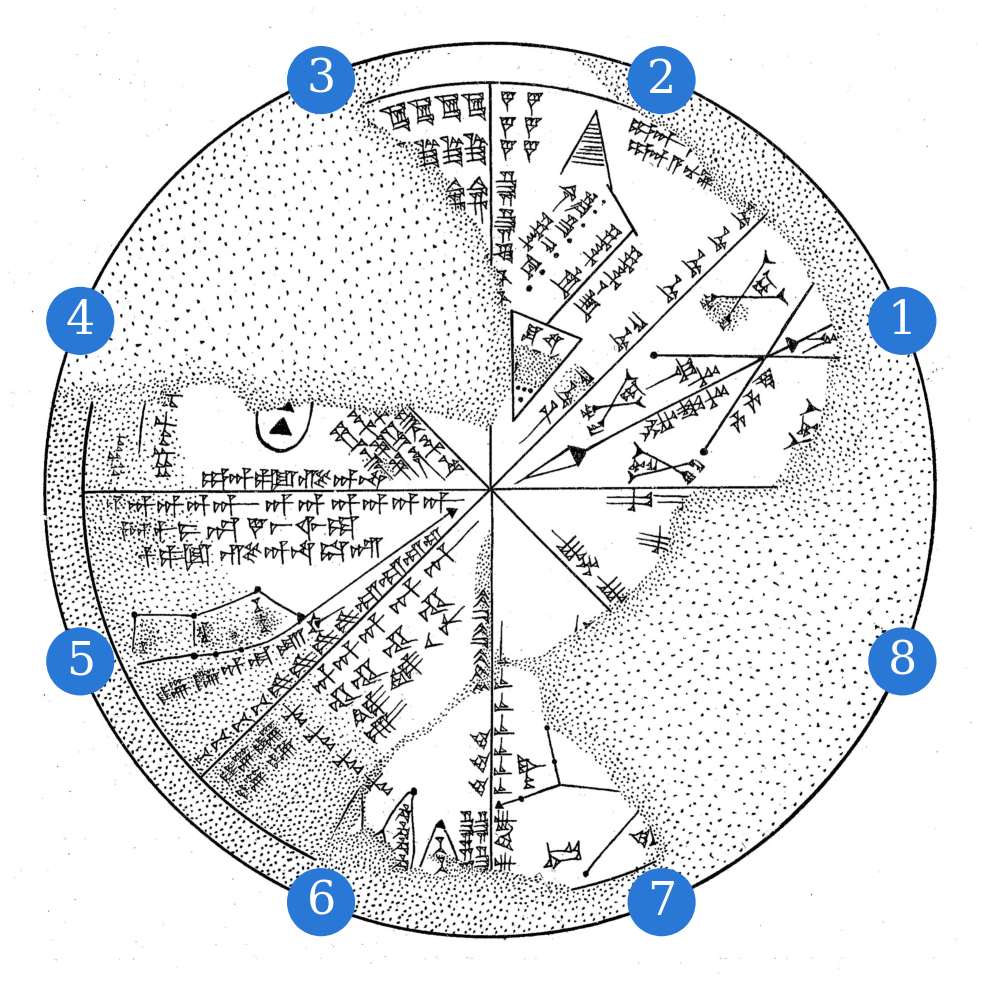
\includegraphics[width=0.56\linewidth]{../figures/fig1-plate.png}
\caption{K\,8538 in King's 1912 copy (\emph{CT}\,33, pl.\,10), with the slice numbering used here.
Weidner's sector $n$ is slice $n+1$.}
\end{figure}

\section{No favourite, only measurement}

The method follows the crib-shift attack used on the Mamari tablet \cite{ross2026}. Each published
reading becomes a rigid mask with only the free settings its author allows. A constellation
identified on the tablet is a crib: the mask places it somewhere on the disc, and the miss is its
angular distance from the slice where the tablet puts it. Each mask is then put through the
identical search on random slice assignments. The score of a reading is the share of random tablets
that fit as well as K\,8538 does.

The cribs are Weidner's identifications: Anunītum (Mirach) and APIN in slice 2, Orion in slice 4, and
the Twins ``who stand in front of Orion'' in slice 5. On these four cribs (Table~\ref{tab:formats}),
both horizon readings and Weidner's own ecliptic order fall well short. The heliacal reading fits
every crib exactly.

\begin{table}[h]
\centering\small
\begin{tabular}{@{}llrr@{}}
\toprule
Reading & Free settings & Total miss & Random tablets fit as well \\
\midrule
Dawn calendar (heliacal rising) & rotation, direction & 0° & \textbf{2.0\%} \\
Koch, one-night horizon & hour, rotation, direction & 0° & 8.7\% \\
Weidner, ecliptic order & rotation, direction & 23.8° & 10.0\% \\
Bosanquet and Sayce, sunset horizon & rotation, direction & 28.9° & 12.7\% \\
\bottomrule
\end{tabular}
\caption{Published readings scored on identical cribs (Weidner's four; 700\,BCE; 150 random tablets).}
\label{tab:formats}
\end{table}

\section{A calendar in the clay}

In the heliacal reading, each constellation is placed by the morning it first rises before dawn,
after weeks lost in the Sun's glare. The eight slices become eighths of the year, about 45 days each.
Mesopotamian administration kept, beside the lunar months of daily life, a schematic year of exactly
360 days used for fiscal and astronomical reckoning \cite{brackbernsen2007}, and MUL.APIN dates its
star risings in that year \cite{hp1989}. Divided by eight, the 360-day year gives periods of exactly
45 days.

\begin{figure}[t]
\centering
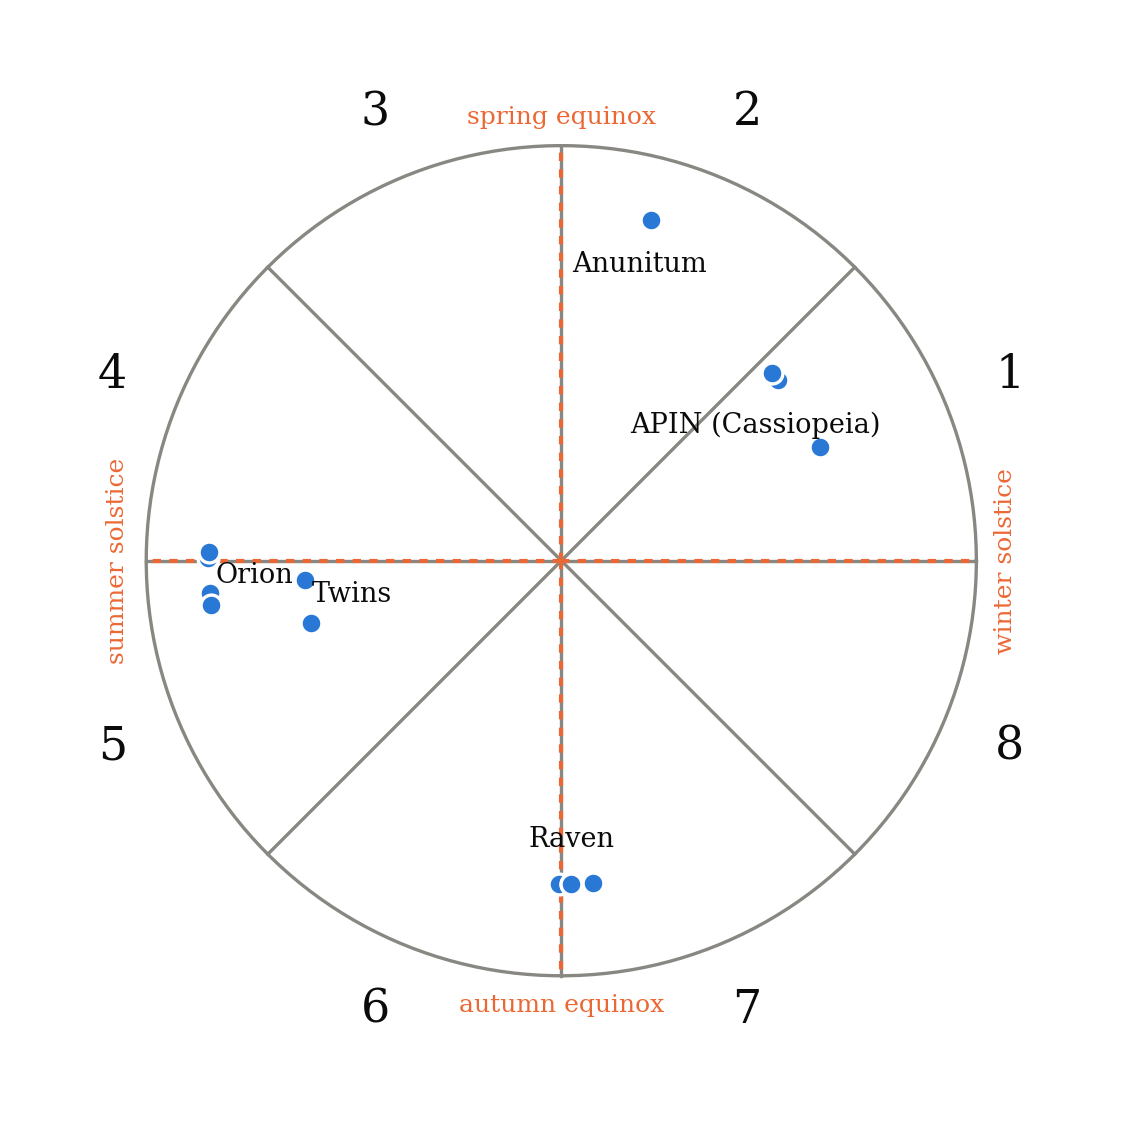
\includegraphics[width=0.52\linewidth]{../figures/fig2-wheel.png}
\caption{The eight slices as the year. Each dot is a crib star's heliacal rising at Nineveh in
700\,BCE, placed by the Sun's longitude that morning; dashed lines mark the solstices and equinoxes.
Slice 1 opens at the winter solstice. APIN (as Cassiopeia) is the one crib that misses, by 3.3°.}
\end{figure}

\section{The breakthrough}

A hypothesis earns trust by predicting what it has not seen. Weidner read a bird in slice 6, four
signs \emph{hu}, \emph{iṣṣūru}, ``perhaps the Raven''. The bird had been used in no fit. Assuming
the calendar, the prediction was written and hashed before computing: the stars of Corvus must rise
at dawn within slice 6. All four did (Figure~\ref{fig:raven}). The fit also places the opening of
slice 1 at the winter solstice, where Weidner had put its figure a century before.

\begin{figure}[h]
\centering
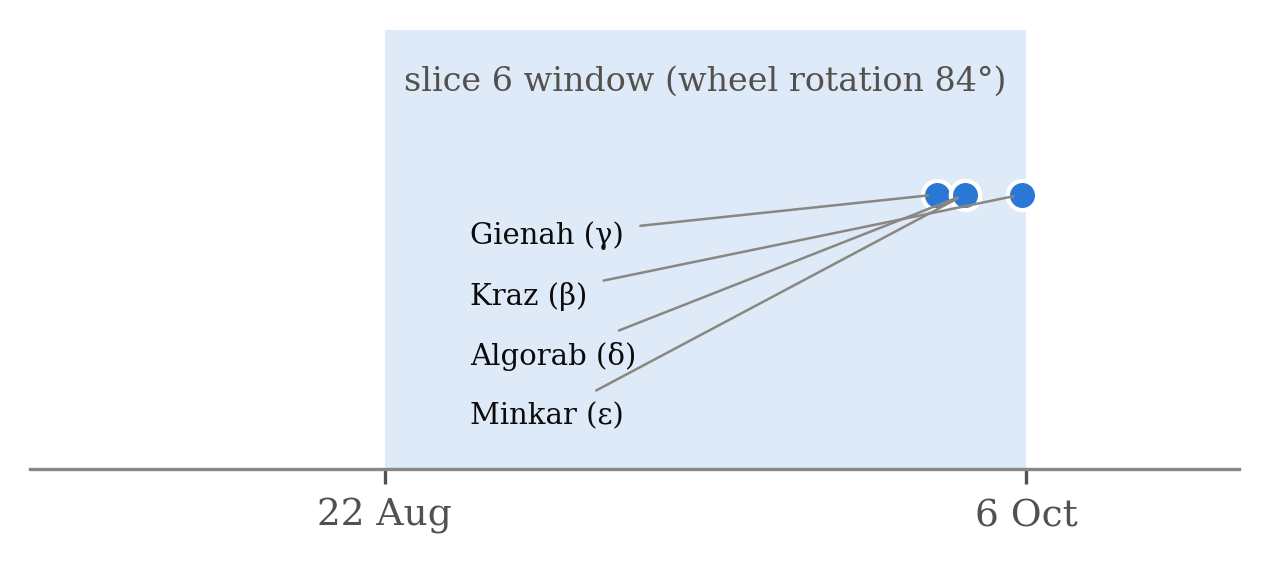
\includegraphics[width=0.72\linewidth]{../figures/fig5-raven.png}
\caption{The locked prediction. Heliacal risings of the four Corvus stars in 700\,BCE (Julian dates)
against the slice-6 window of the wheel fitted on Weidner's other cribs. Kraz sits 0.3° from the edge.}
\label{fig:raven}
\end{figure}

With the Raven as a fifth crib, 64 of 10{,}000 random tablets fit as well as K\,8538: \textbf{0.64\%}
(Figure~\ref{fig:null}). The result is stable across eleven centuries, and no single crib carries it
(Table~\ref{tab:robust}, Figure~\ref{fig:robust}). With APIN taken as Triangulum, the modern
identification, all five cribs fall exactly in their slices, and the result is 0.48\%.

\begin{figure}[t]
\centering
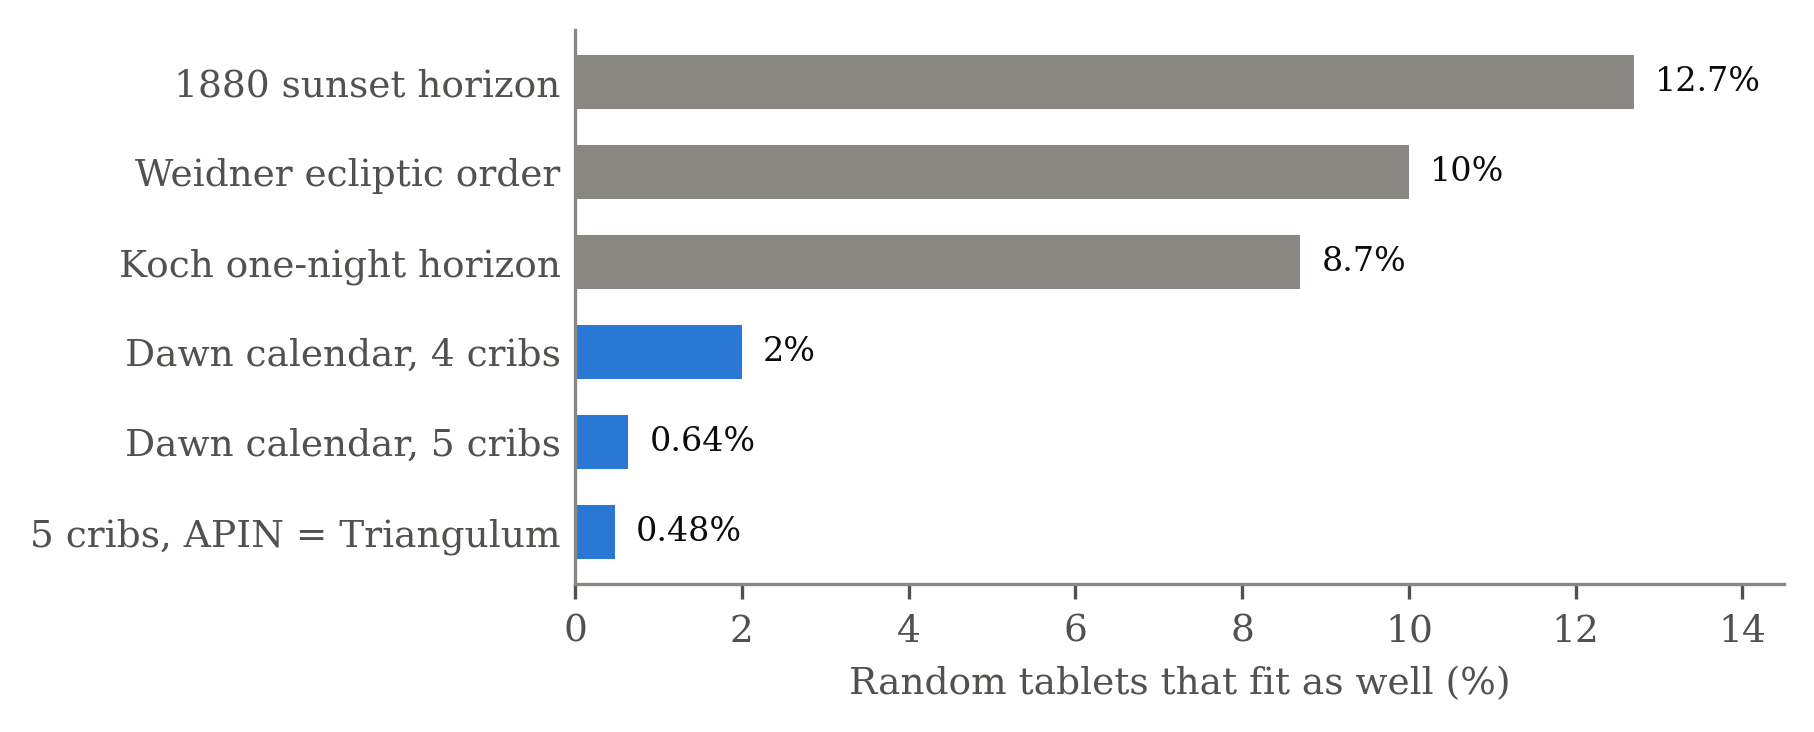
\includegraphics[width=0.78\linewidth]{../figures/fig3-scoreboard.png}
\caption{Share of random tablets that fit as well as K\,8538, by reading. Grey: published readings on
Weidner's four cribs. Blue: the dawn calendar on four cribs, then five.}
\end{figure}

\begin{figure}[t]
\centering
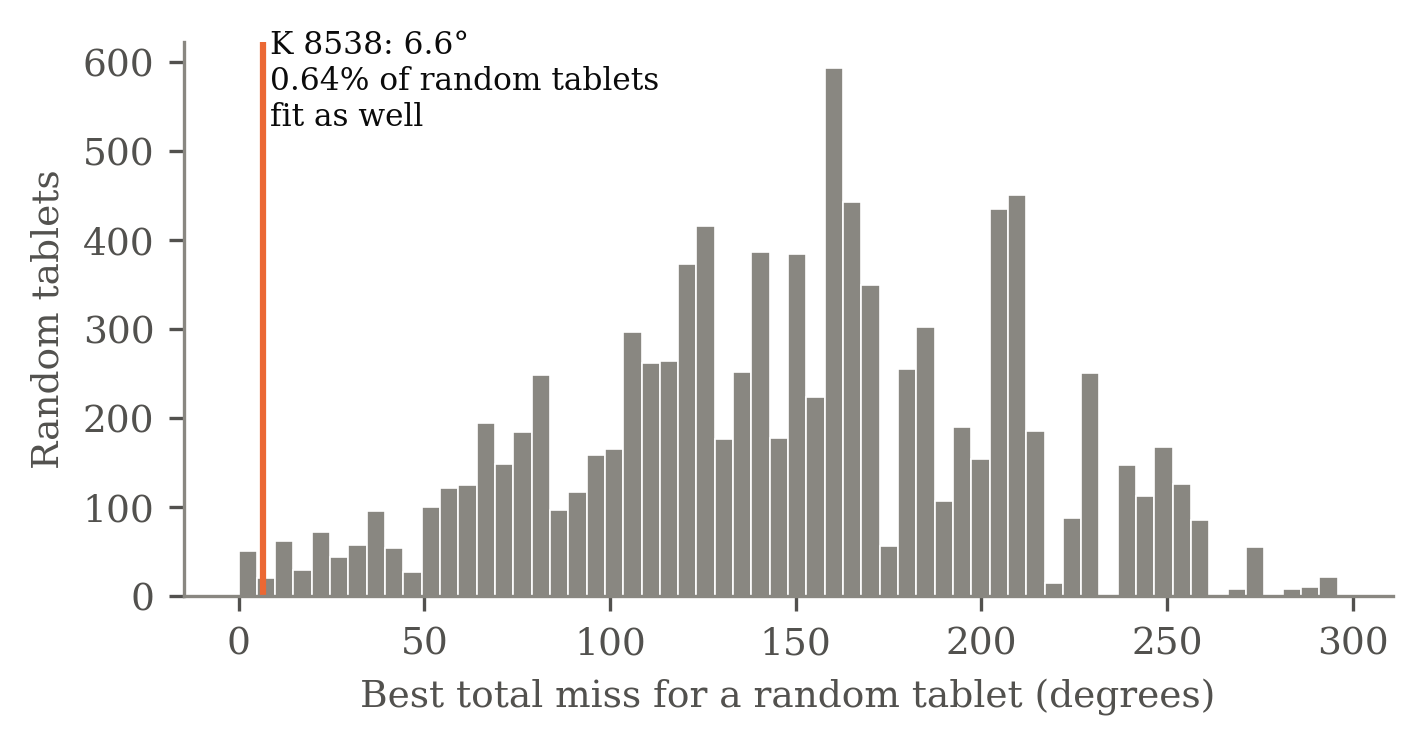
\includegraphics[width=0.78\linewidth]{../figures/fig4-null.png}
\caption{Best total miss for 10{,}000 random tablets under the dawn calendar, five cribs, 700\,BCE.
K\,8538 sits at 6.6°.}
\label{fig:null}
\end{figure}

\begin{table}[h]
\centering\small
\begin{tabular}{@{}lr@{\qquad}lr@{}}
\toprule
Epoch & Random tablets fit as well & Crib dropped & Random tablets fit as well \\
\midrule
1500\,BCE & 0.62\% & Anunītum & 4.33\% \\
1000\,BCE & 0.61\% & APIN & 3.00\% \\
700\,BCE & 0.64\% & Orion & 2.70\% \\
400\,BCE & 0.71\% & Twins & 3.44\% \\
APIN as Triangulum & 0.48\% & Raven & 3.02\% \\
\bottomrule
\end{tabular}
\caption{Robustness, 10{,}000 random tablets each. Slices taken as equal 45-day periods; slices taken
as 45° of the Sun's path give the same results within sampling error.}
\label{tab:robust}
\end{table}

\begin{figure}[t]
\centering
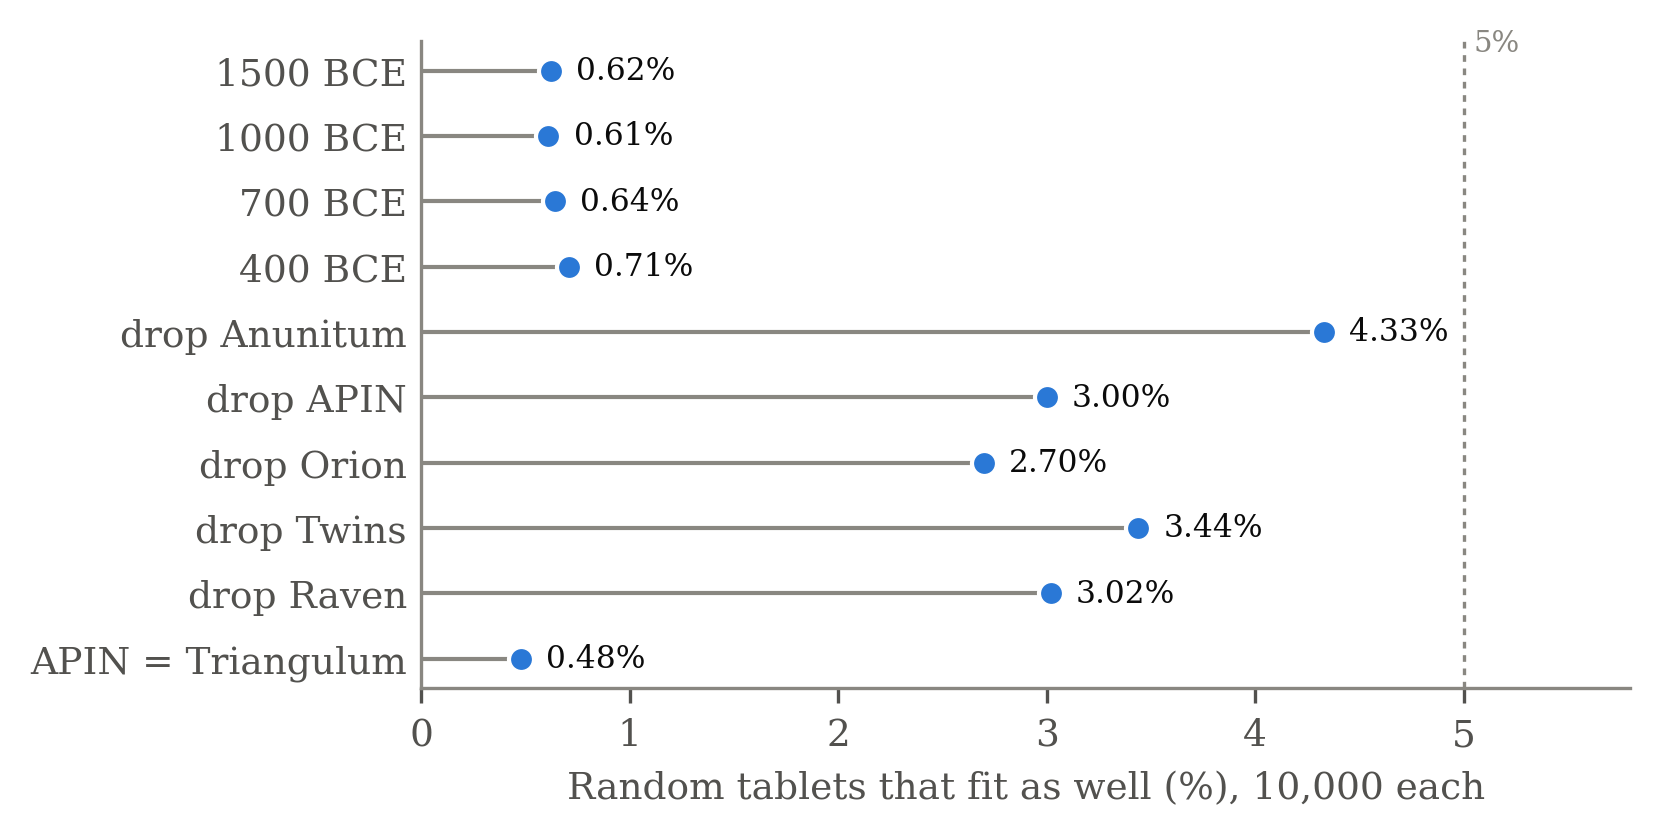
\includegraphics[width=0.78\linewidth]{../figures/fig6-robust.png}
\caption{Robustness by epoch and by leave-one-out.}
\label{fig:robust}
\end{figure}

\section{Interpretation: an administrative calendar}

The measurement supports a reading of K\,8538 as an \textbf{administrative calendar}: eight periods
of 45 days in the 360-day administrative year, each marked by the constellations rising with the
dawn. A count of 360 days falls about five days behind the Sun each year; the dawn stars do not.
Whoever held the disc could look east at first light and know which period had begun.

The reading accounts for features that troubled earlier readers:
\begin{itemize}
\item constellations in the correct order but not in exact positions, because a calendar places stars by date, not by place in the sky;
\item the eight slices, because 360 divided by 8 is 45;
\item the solstice figure of slice 1, and the bird of slice 6;
\item the disagreement of single-night datings by millennia, because heliacal order barely changes over centuries;
\item the absence of any need for a meteor.
\end{itemize}

What the eight periods were for, the deciphered record does not say. Eightfold solar years are known
elsewhere, in the eight nodes of the Chinese year and in the quarter and cross-quarter days of
Britain and Ireland, later used as term days; these show the division is natural, not that it was
practised at Nineveh. The myths fit the wheel in suggestive ways: Weidner places Tiamat and Kingu at
the solstice slice through the astral commentary on \emph{Enūma eliš}; the Tammuz label stands half a
year from the month of Tammuz; and in \emph{Enūma eliš} Marduk orders the year after defeating the storm.
These are offered as how such a calendar might have been taught and remembered. They are
interpretation, not evidence.

The asteroid readings deserve a plain answer. They rest on fitting a single night of sky, which the
known-answer controls show the star layout cannot do, and the Köfels landslide is dated to about
9{,}500 years ago, some 4{,}400 years before Bond and Hempsell's event \cite{nicolussi2015}. The
calendar does not need their object. It does turn their dates into tests: an object seen on
29 June 3123\,BCE would have to sit in slice 4 or 5, and one on 22 September 2193\,BCE in slice 6.

\section{How to break it}

If the calendar is right, each of the following must hold. Any one of them failing refutes it.
\begin{enumerate}
\item The damaged slices name or picture constellations that rise heliacally in their windows: the Hired Man or the Crook in slice 3, the Furrow or Šu.pa in slice 7, the Scorpion or Pabilsag in slice 8.
\item The large figure of slice 1 is a midwinter riser, in the region of Aquarius or Capricorn.
\item The numbers of slice 6, read independently, resolve as fractions of a 45-day period.
\item Any dated sky event claimed on the tablet sits in the slice of its season.
\item Any sister tablet in the same eight-part form shares the heliacal ordering.
\end{enumerate}

\section{Limits}

About seven format variants were tried in all, and the figures above are not corrected for that
search. The Raven was added after it passed its prediction; without it the result is 3.0\%. Five
cribs in four slices is a small set, and the identification of APIN moves the result between 0.48\%
and 0.64\%. The signs come from Weidner's 1915 reading, known here through a machine-read scan, and
from the 1880 drawing; the electronic Babylonian Library, the museum photograph and Koch's monograph
were not read, and an independent transliteration is the largest single gap. The 360-day
administrative year is attested; its division into eight is this paper's reading. The repeated
syllables, the numbers, the large figure, the graded line of seven holes and the three lines meeting
in the first slice remain unexplained. The work has not been peer reviewed.

\section*{Receipts}

Every number in this paper links to a locked rule file, its hash, its code and its output in the
K\,8538 research vault, and every run can be repeated from them. The principal runs are \emph{patchwork-1}
(Table~\ref{tab:formats}), \emph{numbers-and-corvus} (the Raven prediction, rules hash
\texttt{94cc6f7e}), \emph{final-crib-1} (\texttt{21246e2a}) and \emph{robust-1} (\texttt{814c1fe9}).

\section*{Acknowledgements}

First, to the scribes and sky-watchers of Mesopotamia, who watched the dawn, counted the year, and
pressed what they knew into clay that has outlasted every empire since. Then to the author, for
Planisphere, the research system through which this work was carried out.

\begin{thebibliography}{99}\small\setlength{\itemsep}{1pt}
\bibitem{bs1880} R.\,H.\,M. Bosanquet and A.\,H. Sayce, ``The Babylonian Astronomy,'' \emph{Monthly Notices of the Royal Astronomical Society} 40 (1880), 105--123.
\bibitem{king1912} L.\,W. King, \emph{Cuneiform Texts from Babylonian Tablets in the British Museum}, Part XXXIII, pl.\,10 (London, 1912).
\bibitem{weidner1915} E.\,F. Weidner, \emph{Handbuch der babylonischen Astronomie} I (Leipzig, 1915), §o, ``Die Planisphäre K\,8538,'' 107--112.
\bibitem{koch1989} J. Koch, \emph{Neue Untersuchungen zur Topographie des babylonischen Fixsternhimmels} (Wiesbaden, 1989). Not read; cited from secondary reports.
\bibitem{bh2008} A. Bond and M. Hempsell, \emph{A Sumerian Observation of the Köfels' Impact Event} (WritersPrintShop, 2008).
\bibitem{bristol2008} University of Bristol, ``Cuneiform clay tablet translated for the first time,'' press release, 31 March 2008.
\bibitem{sl2019} J. Seifert and F. Lemke, ``The Sumerian K8538 tablet'' and addendum, knowledgeminer.eu (2014, 2019). Known secondhand.
\bibitem{monroe2022} M.\,W. Monroe, ``Astronomical and astrological diagrams from cuneiform sources,'' \emph{Journal for the History of Astronomy} 53 (2022), doi:10.1177/00218286221110919.
\bibitem{cdli} Cuneiform Digital Library Initiative, P397674 (K\,08538).
\bibitem{hp1989} H. Hunger and D. Pingree, \emph{MUL.APIN: An Astronomical Compendium in Cuneiform}, AfO Beiheft 24 (Horn, 1989).
\bibitem{brackbernsen2007} L. Brack-Bernsen, ``The 360-Day Year in Mesopotamia,'' in J.\,M. Steele (ed.), \emph{Calendars and Years} (Oxford, 2007), 83--100.
\bibitem{nicolussi2015} K. Nicolussi et al., ``Precise radiocarbon dating of the giant Köfels landslide (Eastern Alps, Austria),'' \emph{Geomorphology} (2015).
\bibitem{swisseph} Astrodienst, Swiss Ephemeris 2.10.03.
\bibitem{de441} R.\,S. Park et al., ``The JPL Planetary and Lunar Ephemerides DE440 and DE441,'' \emph{Astronomical Journal} 161 (2021), 105.
\bibitem{ross2026} L.\,C. Ross, \emph{Reading Rongorongo}, v2 (2026), Zenodo, doi:10.5281/zenodo.19362491.
\end{thebibliography}
\end{document}
